% !TeX root = Theo_IV.tex

\usepackage{tikz}
%\usepackage{pgfplots}
%\pgfplotsset{compat=1.18}

\usetikzlibrary{
    arrows.meta,
    bending,
    positioning,
    decorations.markings,
    intersections,
    calc,
    decorations.pathreplacing,
    decorations.pathmorphing,
    patterns
}
%\tikzexternalize[prefix=figures/,shell escape=-enable-write18] % activate

\tikzset{
    % Colors
    object color/.style={blue!40!black!80!white},
    object style/.style={object color,thick},
    nice green/.style={green!50!black},
    nice orange/.style={red!60!yellow!70!black!90!white},
    nice dark blue/.style={blue!50!black},
    nice light blue/.style={blue!60!white!70!black},
    nice turquoise/.style={blue!50!green},
    polarisation color/.style={purple},
    charge color/.style={blue!50!white!70!black},
    red laser/.style={red!70!black},
    moving system color/.style={blue!60!black!70!white},
    %
    % Coordinate system
    coordsystem/.style={very thin, color=#1!50},
    xlabel/.style={anchor=north west},
    ylabel/.style={anchor=south east},
    %
    % Nodes and points
    invisible point/.style={circle,inner sep=0pt,outer sep=0pt,minimum size=0pt},
    point/.style={invisible point,fill=black,minimum size=4pt},
    %
    % Arrows
    arrow tip/.tip={Stealth},
    arr/.style={->,>={arrow tip}},
    rarr/.style={<-,>={arrow tip}},
    midarrow/.style={postaction=decorate,decoration={markings, mark=at position #1 with {\arrow[xshift=2.5pt]{arrow tip}}} },
    midarrow/.default=.5,
    rmidarrow/.style={postaction=decorate,decoration={markings, mark=at position #1 with {\arrowreversed{arrow tip}}} },
    rmidarrow/.default=.5,
    distance marker/.style={|<->|,>={arrow tip}},
    %
    % Thermodynamics stuff
    piston bar/.style={line width=2pt},
    piston/.style={line width=8pt}
}
\tikzstyle{every node}=[font=\footnotesize]


\newcommand{\tfigTitel}{
    
\begin{tikzpicture}
        \pgfmathsetmacro{\shadowangle}{132}
        \newlength{\shadowdistance}
        \pgfmathsetlength{\shadowdistance}{0.1ex}
        \pgfmathsetmacro{\shadowopacity}{1}
        \pgfmathsetmacro{\shadowspread}{0.003}
        \pgfmathsetmacro{\shadowsize}{5}
        \pgfmathtruncatemacro{\totshadow}{100}
        \path[nice dark blue,opacity={\shadowopacity/\totshadow},shift={({132-180}:\shadowdistance)},scale={1+\shadowsize}] 
        foreach \nshadow [evaluate=\nshadow as \angshadow using \nshadow/\totshadow*360] in {1,...,\totshadow}{
            node[align=center] at (\angshadow:\shadowspread) {\huge Theoretische Physik 4\\ \\ \\
            \Large Thermodynamik/Statistische Physik}
            };
        \node[align=center] at (0,0) {\huge Theoretische Physik 4\\ \\ \\ \Large Thermodynamik/Statistische Physik};
    \end{tikzpicture}
}

% 100 particles in a rectangular box
\newcommand{\tfigSystemWithManyParticles}{
    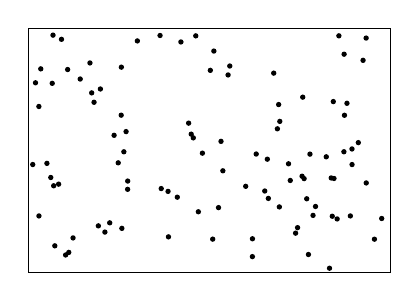
\begin{tikzpicture}[scale=1.5]
        \draw (-1pt,-1pt) rectangle ($(3,2)+(1pt,1pt)$);
        \pgfmathsetseed{1}
        \foreach \i in {1,2,...,100}{
            \draw[fill=black] (rnd*3,rnd*2) circle[radius=.5pt];
        };
    \end{tikzpicture}
}

% Two chambers separated by a piston
\newcommand{\tfigTwoChambersSeparatedByPiston}{
    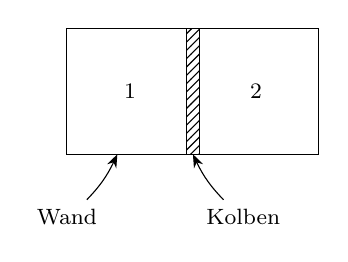
\begin{tikzpicture}[scale=1.6]
        \draw (0,0) rectangle (2,1);
        \node at (.5,.5) {1};
        \node at (1.5,.5) {2};
        \draw[pattern=north east lines] (.95,0) rectangle (1.05,1);
        \node at (0,-.5) {Wand} edge[arr,bend right=10] (.4,0);
        \node at (1.4,-.5) {Kolben} edge[arr,bend left=10] (1,0);
    \end{tikzpicture}
}

% Rectangular box with piston
\newcommand{\tfigRectangularBoxWithPiston}{
    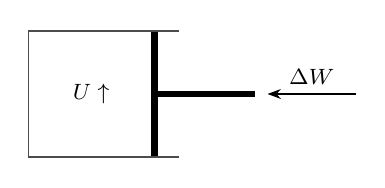
\begin{tikzpicture}[scale=1.6]
        \draw[line width=2.4pt] (1,0) -- (1,1);
        \draw[line width=2pt] (1,.5) -- +(.8,0);
        \draw[rarr] (1.9,.5) -- +(.7,0) node[midway, above] {$\Delta W$};
        \node at (.5,.5) {$U\uparrow$};
        \draw[draw=black!70!white] (1.2,0) -- (0,0) -- (0,1) -- (1.2,1);
    \end{tikzpicture}
}

% Water with ice cubes. Stiring heats up the water and ice cubes vanish
\newcommand{\tfigWaterStiringIceCubes}{
    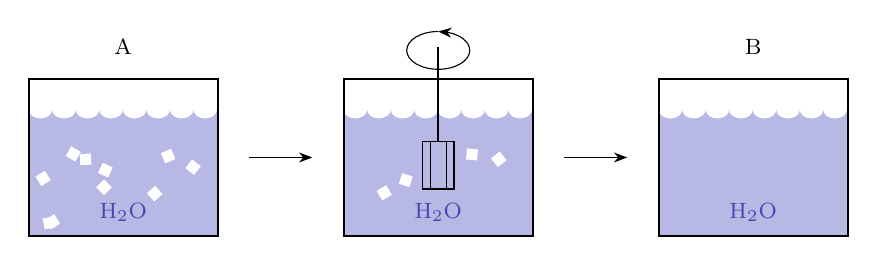
\begin{tikzpicture}[water color/.style={nice light blue},wave deco/.style={decoration={bumps,amplitude=-3,segment length=17}},scale=2]
        \begin{scope}
            \fill[blue!20!white!90!black] decorate[wave deco] {(0,.8) -- (1.2,.8)} -- (1.2,0) -- (0,0) -- (0,.8);
            \draw[thick] (0,0) rectangle (1.2,1); 
            \pgfmathsetseed{5}
            \foreach \i in {1,2,...,10} {
                \coordinate (A) at (rnd+.1,rnd*.5+.1);
                \fill[color=white,rotate around={rnd*360:(A)}] (A) rectangle +(2pt,2pt);
            };
            \node[water color] at (.6,.15) {$\mathrm{H}_2\mathrm{O}$};
            \node at (.6,1.2) {A};
        \end{scope}
        \draw[arr] (1.4,.5) -- +(.4,0); 
        \begin{scope}[xshift=2cm]
            \fill[blue!20!white!90!black] decorate[wave deco] {(0,.8) -- (1.2,.8)} -- (1.2,0) -- (0,0) -- (0,.8);
            \draw[thick] (0,0) rectangle (1.2,1); 
            \foreach \i in {1,2,...,4} {
                \coordinate (A) at (rnd+.1,rnd*.5+.1);
                \fill[color=white,rotate around={rnd*360:(A)}] (A) rectangle +(2pt,2pt);
            };
            \node[water color] at (.6,.15) {$\mathrm{H}_2\mathrm{O}$};
            
            \draw (.5,.3) rectangle +(.2,.3) (.55,.3) rectangle +(.1,.3);
            \draw[thick] (.6,.6)-- +(0,.6);
            \draw[arr] (.6,1.3) arc[x radius=.2, y radius=.12,start angle=-270, end angle=90];
        \end{scope}
        \draw[arr] (3.4,.5) -- +(.4,0); 
        \begin{scope}[xshift=4cm]
            \fill[blue!20!white!90!black] decorate[wave deco] {(0,.8) -- (1.2,.8)} -- (1.2,0) -- (0,0) -- (0,.8);
            \draw[thick] (0,0) rectangle (1.2,1);
            \node[water color] at (.6,.15) {$\mathrm{H}_2\mathrm{O}$};
            \node at (.6,1.2) {B};
        \end{scope}
    \end{tikzpicture}
}

% Visualize that W,Q are no state functions. Adding different ratios of W and Q to a system may lead to the same inner energy U. 
\newcommand{\tfigWQAreNoStateFunctions}{
    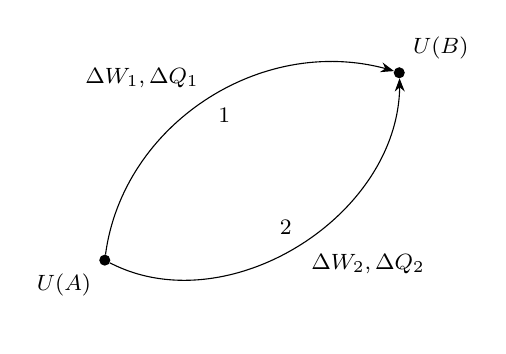
\begin{tikzpicture}[scale=1.7]
        \node[point,label={north east}:$U(B)$] (Point B) at (2.2,1.4) {};
        \node[point,label={south west}:$U(A)$] (Point A) at (0,0) {} 
        edge[arr,bend left=50] node[midway, anchor=south east] {$\Delta W_1,\Delta Q_1$} node[midway, anchor=north west] {1} (Point B)
        edge[arr,bend right=60] node[midway, anchor=north west] {$\Delta W_2,\Delta Q_2$} node[midway, anchor=south east] {2} (Point B);
    \end{tikzpicture}
}

% Sketch of fundamental relations between inner energy and entropy.
\newcommand{\tfigSchemaFundamentalbeziehung}{    
    \begin{tikzpicture}[scale=1.5]
        \draw[arr] (0,0) node[anchor=north] {$0$} -- (0,2) node[ylabel] {$U$};
        \draw[arr] (0,0) -- (3,0) node[xlabel] {$S$};
        \draw[nice light blue] (0,1) .. controls +(0:1.2) and +(-135:.7) .. (2.5,1.8);
        \begin{scope}[xshift=4.5cm]
            \draw[arr] (0,0) node[anchor=north] {$0$} -- (0,2) node[ylabel] {$S$};
            \draw[arr] (0,0) -- (3,0) node[xlabel] {$U$};
            \draw[nice light blue] (1,0) .. controls +(90:.8) and +(-165:.7) .. (2.8,1.8);
        \end{scope}
    \end{tikzpicture}
}

% System with two subsystems separated by an impermeable and fixed but thermally conductive wall. 
\newcommand{\tfigDoppelsystemUSfesteWaermeleitendeWand}{
    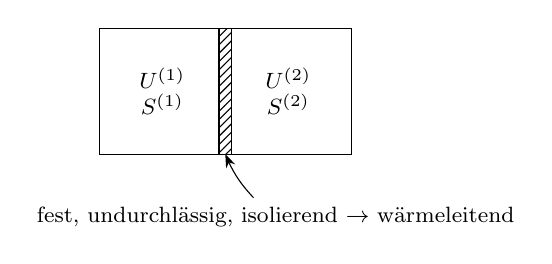
\begin{tikzpicture}[scale=1.6]
        \draw (0,0) rectangle (2,1);
        \node[align=center] at (.5,.5) {$U^{(1)}$\\$S^{(1)}$};
        \node[align=center] at (1.5,.5) {$U^{(2)}$\\$S^{(2)}$};
        \draw[pattern=north east lines] (.95,0) rectangle (1.05,1);
        \node at (1.4,-.5) {fest, undurchlässig, isolierend $\rightarrow$ wärmeleitend} edge[arr,bend left=10] (1,0);
    \end{tikzpicture}
}

% System with two subsystems separated by an impermeable but movable and thermally conductive wall. 
\newcommand{\tfigDoppelsystemUVNbeweglicheWaermeleitendeWand}{
    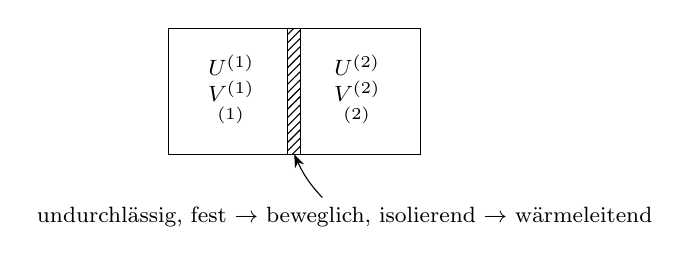
\begin{tikzpicture}[scale=1.6]
        \draw (0,0) rectangle (2,1);
        \node[align=center] at (.5,.5) {$U^{(1)}$\\$V^{(1)}$\\$\sm^{(1)}$};
        \node[align=center] at (1.5,.5) {$U^{(2)}$\\$V^{(2)}$\\$\sm^{(2)}$};
        \draw[pattern=north east lines] (.95,0) rectangle (1.05,1);
        \node at (1.4,-.5) {undurchlässig, fest $\rightarrow$ beweglich, isolierend $\rightarrow$ wärmeleitend} edge[arr,bend left=10] (1,0);
    \end{tikzpicture}
}

% Function U(S) with maximum. 
\newcommand{\tfigFunktionEntropieMaximum}{
    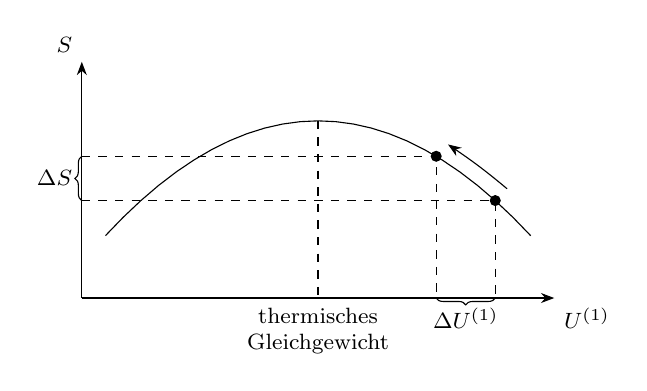
\begin{tikzpicture}[scale=1.5]
        \draw[arr] (0,0) -- (0,2) node[ylabel] {$S$};
        \draw[arr] (0,0) -- (4,0) node[xlabel] {$U^{(1)}$};
        
        \path let \n{thermisches GG}={2}, \n{x1}={3},\n{x2}={3.5},\n{y1}={-.3*(\n{x1}-\n{thermisches GG})^2+1.5},\n{y2}={-.3*(\n{x2}-\n{thermisches GG})^2+1.5} in        
        coordinate (P1) at (\n{x1},\n{y1})
        coordinate (P2) at (\n{x2},\n{y2});
        \node[point] at (P1) {};
        \node[point] at (P2) {};
        \draw let \n{thermisches GG}={2} in plot[domain=.2:3.8] (\x,{-.3*(\x-\n{thermisches GG})^2+1.5});
        \draw[dashed] let \n{thermisches GG}={2},\p1=(P1),\p2=(P2) in 
        (\n{thermisches GG},1.5) -- +(0,-1.5) node[below,align=center] {thermisches\\Gleichgewicht}
        (0,\y1) -- (P1) -- (\x1,0) (0,\y2) -- (P2) -- (\x2,0);
        \draw[decorate, decoration = {brace}] let \p1=(P1),\p2=(P2) in
        (0,\y2)  --(0,\y1) node[midway,left]{$\Delta S$};
        \draw[decorate, decoration = {brace}] let \p1=(P1),\p2=(P2) in
        (\x2,0)  --(\x1,0) node[midway,below]{$\Delta U^{(1)}$};
        
        \draw[arr] ([shift={(.1,.1)}]P2)to[bend right=3] ([shift={(.1,.1)}]P1);
    \end{tikzpicture}
}


% System with two subsystems separated by a fixed but semipermeable and thermally conductive wall. 
\newcommand{\tfigDoppelsystemUVNbeweglicheIsolierendeWand}{
    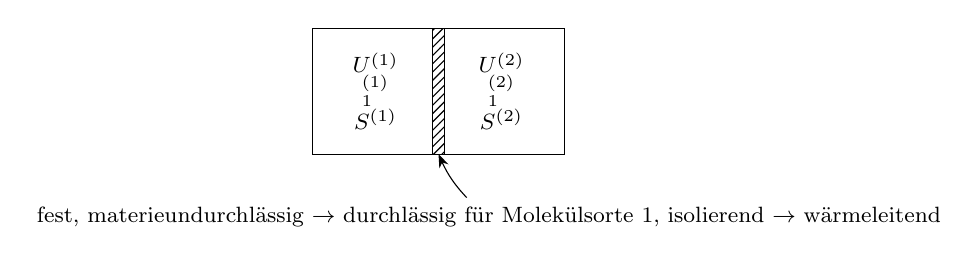
\begin{tikzpicture}[scale=1.6]
        \draw (0,0) rectangle (2,1);
        \node[align=center] at (.5,.5) {$U^{(1)}$\\$\sm_1^{(1)}$\\$S^{(1)}$};
        \node[align=center] at (1.5,.5) {$U^{(2)}$\\$\sm_1^{(2)}$\\$S^{(2)}$};
        \draw[pattern=north east lines] (.95,0) rectangle (1.05,1);
        \node at (1.4,-.5) {fest, materieundurchlässig $\rightarrow$ durchlässig für Molekülsorte 1, isolierend $\rightarrow$ wärmeleitend} edge[arr,bend left=10] (1,0);
    \end{tikzpicture}
}


% Degeneracy function g(n,N) for N >> 1 (gaussian approximation)
\newcommand{\tfigDegeneracyFunctionGauss}{
    \begin{tikzpicture}[scale=4]
        \draw[arr] (-.7,0) -- (.7,0) node[xlabel] {$\frac{n}{N}$};
        %\draw[arr] (0,0) -- (0,1) node[ylabel] {$g(n,N)$};
        
        \draw let \n{N}={10} in plot[domain=-.5:.5,smooth,yscale=.003] (\x,{sqrt(2/(3.14159*\n{N}))*2^\n{N}*exp(-2*(\x*\n{N})^2/\n{N})}) 
        coordinate (P) at ({sqrt(1/(2*\n{N}))},{.003*sqrt(2/(3.14159*\n{N}))*2^\n{N}/exp(1)});
        \draw (-.5,.02) -- +(0,-.04) node[below] {$-\frac{1}{2}$}(.5,.02) -- +(0,-.04) node[below] {$\frac{1}{2}$};
        \draw[dashed] let \p1=(P) in (-\x1,0) -- (-\x1,\y1) -- (\x1,\y1) -- (\x1,0); 
        
        \draw[decoration={brace},decorate] let \p1=(P) in (\x1,-.02) -- +(-\x1,0) node[midway, below,yshift=-.04cm] {$\frac{n_n}{N}$};
    \end{tikzpicture}
}


% (1) System with two subsystems and wall, one filled with particles
% (2) barrier opened
\newcommand{\tfigTwoSubsystemsParticlesRemoveWall}{
    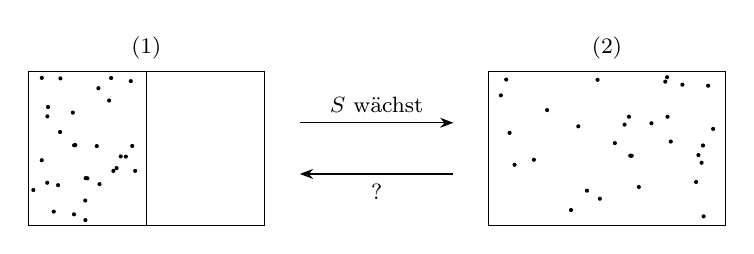
\begin{tikzpicture}[scale=1.5]
        \draw (0,0) rectangle (2, 1.3);
        \node at (1,1.5) {(1)};
        \draw (1,0) -- (1,1.3);
        \pgfmathsetseed{2}
        \foreach \n in {1,...,30}{
            \fill (.02+rnd*0.96,.02+rnd*1.26) circle[radius=.5pt];
        }
        
        \draw[arr] (2.3,1.3*2/3) -- +(1.3,0) node[midway, above] {$S$ wächst};
        \draw[rarr] (2.3,1.3/3) -- +(1.3,0) node[midway, below] {?};
        
        \begin{scope}[xshift=3.9cm]
            \node at (1,1.5) {(2)};
            \draw (0,0) rectangle (2, 1.3);
            \pgfmathsetseed{3}
            \foreach \n in {1,...,30}{
                \fill (.02+rnd*1.96,.02+rnd*1.26) circle[radius=.5pt];
            }
        \end{scope}
    \end{tikzpicture}
}


% Degeneracy function for large systems -> delta function
\newcommand{\tfigDegeneracyFunctionLargeSystemsDelta}{
    \begin{tikzpicture}[scale=4]
        \draw[arr] (-.7,0) -- (.7,0) node[xlabel] {$\frac{n_1}{N_1}$};
        \draw[arr] (0,0) -- (0,.7) node[ylabel] {$(g_1g_2)(n_1)$};
        \draw (-.5,.5pt) -- +(0,-1pt) node[below] {$-\frac{1}{2}$};
        \draw (.5,.5pt) -- +(0,-1pt) node[below] {$\frac{1}{2}$};
        \draw[nice green] (.2,.5) -- (.2,0) node[near start, right] {$\frac{\delta_n}{N_1}=10^{-11}$}
        node[below,black] {$\frac{\hat{n}_1}{N_1}$};
        \draw (.5pt,.5) -- (-.5pt,.5) node[left] {$(g_1g_2)_\mathrm{max}$};
    \end{tikzpicture}
}

% Placeholder
\newcommand{\tfigPlaceholder}{
    \begin{tikzpicture}
        \filldraw[fill=formalshade] (0,0) rectangle (3,3) ;
        \node[black] at (1.5,1.5){\textbf{?}};
    \end{tikzpicture}
}

% Reversible vs. irreversible Processes and quasistationary vs. non-stationary 
\newcommand{\tfigProcessReversibleQuasistationary}{
    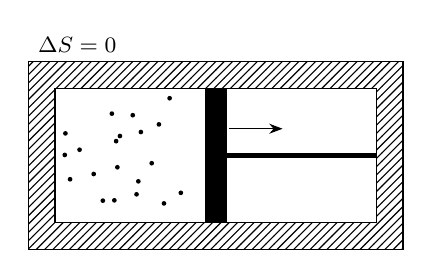
\begin{tikzpicture}[scale=1.7]
        \draw[piston] (0,0) -- (0,1);
        \draw[piston bar] (0,.5) -- (1.2,.5);
        \draw[arr] (.1,.7) -- +(.4,0);
        \draw[pattern=north east lines,even odd rule] (-1.4,1.2) rectangle (1.4,-.2) node[pos=0,anchor=south west] {$\Delta S=0$} (-1.2,0) rectangle (1.2,1);
        \pgfmathsetseed{16}
        \foreach \n in {1,...,20}{
            \fill (.02-1.2+rnd*.96,.02+rnd*.96) circle[radius=.5pt];
        }
    \end{tikzpicture}
}
            
\newcommand{\tfigProcessIrreversibleQuasistationary}{
    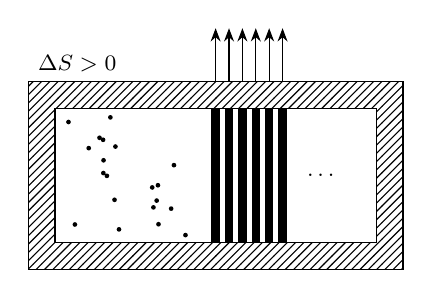
\begin{tikzpicture}[scale=1.7]
        \foreach \x in {0,.1,...,.6}{
            \draw[line width=3pt] (\x,0) -- +(0,1);
            \draw[arr] (\x,1.2) -- +(0,.4);
        }
        \node at (.8,.5) {\ldots};
        \draw[pattern=north east lines,even odd rule] (-1.4,1.2) rectangle (1.4,-.2) node[pos=0,anchor=south west] {$\Delta S>0$} (-1.2,0) rectangle (1.2,1);
        \pgfmathsetseed{30}
        \foreach \n in {1,...,20}{
            \fill (.02-1.2+rnd*.96,.04+rnd*.90) circle[radius=.5pt];
        }
    \end{tikzpicture}
}

\newcommand{\tfigProcessIrreversibleNonquasistationary}{
    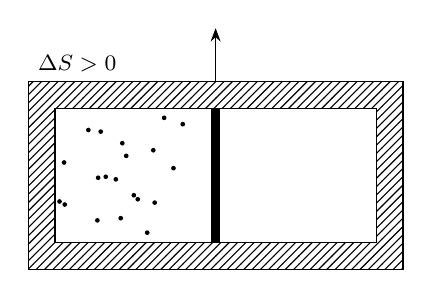
\begin{tikzpicture}[scale=1.7]
        \draw[line width=3pt] (0,0) -- +(0,1);
        \draw[arr] (0,1.2) -- +(0,.4);
        
        \draw[pattern=north east lines,even odd rule] (-1.4,1.2) rectangle (1.4,-.2) node[pos=0,anchor=south west] {$\Delta S>0$} (-1.2,0) rectangle (1.2,1);
        \pgfmathsetseed{29}
        \foreach \n in {1,...,20}{
            \fill (.02-1.2+rnd*.96,.02+rnd*.96) circle[radius=.5pt];
        }
    \end{tikzpicture}
}

% Mixing od two gases 
\newcommand{\tfigMixTwoGases}{
    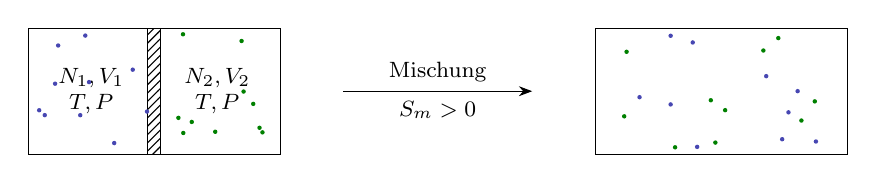
\begin{tikzpicture}[scale=1.6]
        \draw (-1,0) rectangle (1,1);
        \node[align=center] at (-.5,.5) {$N_1,V_1$\\$T,P$};
        \node[align=center] at (.5,.5) {$N_2,V_2$\\$T,P$};
        \draw[pattern=north east lines] (-.05,0) rectangle (.05,1);
        \pgfmathsetseed{228}
        \foreach \n in {1,...,10}{
            \fill[nice light blue] (.02-1+rnd*0.96,.02+rnd*0.96) circle[radius=.5pt];
            \fill[nice green] (.02+rnd*0.96,.02+rnd*0.96) circle[radius=.5pt];
        }
    
        \draw[arr] (1.5,.5) -- +(1.5,0) node[midway, above] {Mischung} node[midway, below]{$S_m>0$}; 
        
        \begin{scope}[xshift=4.5cm]
            \draw (-1,0) rectangle (1,1);
            \pgfmathsetseed{223}
            \foreach \n in {1,...,10}{
                \fill[nice light blue] (.02-1+rnd*1.96,.04+rnd*0.92) circle[radius=.5pt];
                \fill[nice green] (.02-1+rnd*1.96,.04+rnd*0.92) circle[radius=.5pt];
            }
        \end{scope}
    \end{tikzpicture}
}

% Thawing of degrees of freedom: translation, rotation, vibration
\newcommand{\tfigThawingOfDegreesOfFreedom}{
    \begin{tikzpicture}
        \draw[arr] (0,0) -- (0,4.5) node[ylabel] {$c_v/R$};
        \draw[arr] (0,0) -- (9,0) node[xlabel] {$T$};
    
        \draw (0,3/2) -- +(-2pt,0) node[left] {$\frac32$};
        \draw (0,5/2) -- +(-2pt,0) node[left]{$\frac52$};
        \draw (0,7/2) -- +(-2pt,0) node[left] {$\frac72$};
        \draw[decoration={brace}, decorate] (-.5,0) -- (-.5,3/2) node[midway, left,xshift=-2mm] {flüssig/fest};
        \draw[decoration={brace}, decorate] (-.5,3/2) -- (-.5,7/2) node[midway, left,xshift=-2mm] {gasförmig};
        \draw[dashed] (0,3/2) -- +(8.5,0);
        \draw[dashed] (0,5/2) -- +(8.5,0);
        \draw[dashed] (0,7/2) -- +(8.5,0);
    
        \draw (0,0) .. controls +(10:1) and +(-135:1) .. (2,3/4) .. controls +(45:.5) and +(-180:.5) .. (3,3/2) -- (4,3/2) node[midway, above] {Translation}  .. controls +(0:.5) and +(-180:.5) .. (5,5/2) -- (6,5/2) node[midway, above] {Rotation} .. controls +(0:.5) and +(-180:.5) .. (7,7/2) -- +(1.5,0) node[midway, above] {Schwingung};
    \end{tikzpicture}
}

% Adiabatic gas-compression 
\newcommand{\tfigAdiabaticGasCompression}{
    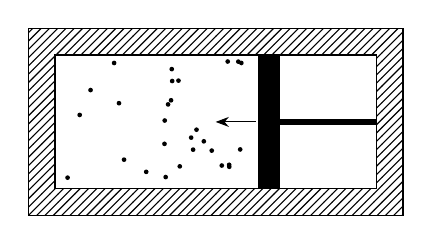
\begin{tikzpicture}[scale=1.7]
        \draw[piston] (.4,0) -- (.4,1);
        \draw[piston bar] (.4,.5) -- (1.2,.5);
        \draw[arr] (.3,.5) -- (0,.5);
        \draw[pattern=north east lines,even odd rule] (-1.4,1.2) rectangle (1.4,-.2)  (-1.2,0) rectangle (1.2,1);
        \pgfmathsetseed{13}
        \foreach \n in {1,...,28}{
            \fill (-1.15+rnd*1.4,.02+rnd*.96) circle[radius=.5pt];
        }
    \end{tikzpicture}
}

% Mixing-Machine (First state)
\newcommand{\tfigMixingMachineOne}{
    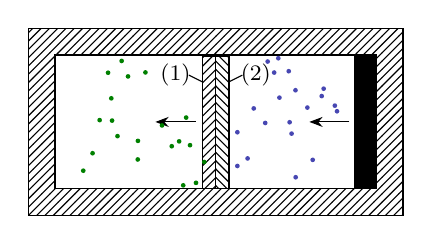
\begin{tikzpicture}[scale=1.7]
        \draw[piston] (1.12,0) -- (1.12,1);
        %\draw[piston bar] (0,.5) -- (1.2,.5);
        \draw[arr] (1,.5) -- (.7,.5);
        \draw[arr] (-.15,.5) -- (-.45,.5);
        \draw[pattern=north west lines,even odd rule] (0,-0) rectangle (0.1,.99);
        \node at (.3,.85){(2)} ;
        \draw[black](.2,.85)-- (.1,.8);
        \node at (-.3,.85){(1)} ;
        \draw[black](-.2,.85)-- (-.1,.8);
        \draw[pattern=north east lines,even odd rule] (-.1,-0) rectangle (0,.99);
        \draw[pattern=north east lines,even odd rule] (-1.4,1.2) rectangle (1.4,-.2)  (-1.2,0) rectangle (1.2,1);
        \pgfmathsetseed{9}
        \foreach \n in {1,...,20}{
            \fill[nice green] (-1.05+rnd*.97,.02+rnd*.95) circle[radius=.5pt];
        }
        \pgfmathsetseed{20}
        \foreach \n in {1,...,20}{
            \fill[nice light blue] (.05+rnd*.87,.02+rnd*.96) circle[radius=.5pt];
        }
    \end{tikzpicture}
}

% Mixing-Machine (Second state)
\newcommand{\tfigMixingMachineTwo}{
    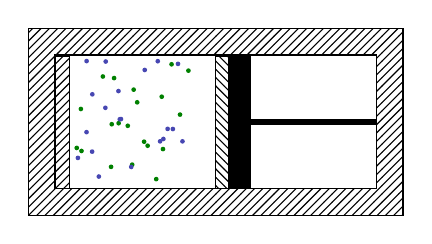
\begin{tikzpicture}[scale=1.7]
        \draw[piston] (0.18,0) -- (0.18,1);
        \draw[piston bar] (0.19,.5) -- (1.2,.5);
        %\draw[arr] (.3,.5) -- (0,.5);
        \draw[pattern=north west lines,even odd rule] (0,-0) rectangle (0.1,.99);
        \draw[pattern=north east lines,even odd rule] (-1.2,-0) rectangle (-1.09,.99);
        \draw[pattern=north east lines,even odd rule] (-1.4,1.2) rectangle (1.4,-.2)  (-1.2,0) rectangle (1.2,1);
        \pgfmathsetseed{29}
        \foreach \n in {1,...,20}{
            \fill[nice green] (-1.05+rnd*.87,.02+rnd*.96) circle[radius=.5pt];
        }
        \pgfmathsetseed{2}
        \foreach \n in {1,...,20}{
            \fill[nice light blue] (-1.05+rnd*.87,.02+rnd*.96) circle[radius=.5pt];
        }
    \end{tikzpicture}
}

% Maximized work in a coupled system
\newcommand{\tfigTheoremMaximizedWork}{
    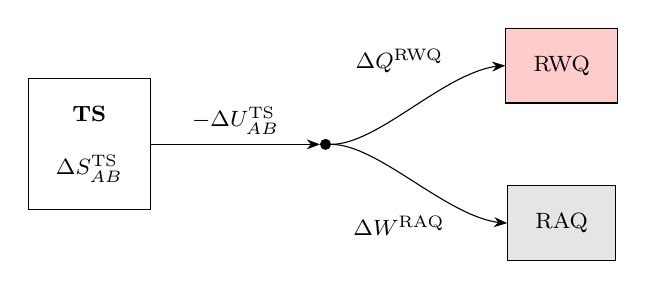
\begin{tikzpicture}
        [
            system node/.style={rectangle,draw,inner sep=10pt}
        ]
        \node[system node, fill=red!20!white] (RWQ) at (3,1) {RWQ};
        \node[system node, fill=black!10!white] (RAQ) at (3,-1) {RAQ};
        \node[point] (P) at (0,0) {};
        \draw[arr] (P) .. controls +(0:.7) and +(180:.7) .. (RAQ.west) node[pos=.7,anchor=north east] {$\Delta W^\mathrm{RAQ}$};
        \draw[arr] (P) .. controls +(0:.7) and +(180:.7) .. (RWQ.west) node[pos=.7,anchor=south east] {$\Delta Q^\mathrm{RWQ}$};
        edge[arr] (RWQ) 
        edge[arr] (RAQ);
        \node[system node,align=center] at (-3,0) {\textbf{TS}\\\\$\Delta S_{AB}^\mathrm{TS}$} edge[arr] node[midway, above] {$-\Delta U_{AB}^\mathrm{TS}$} (P);
    \end{tikzpicture}
}

% Maximized work in a coupled system
\newcommand{\tfigThermodynamicMaschine}{
    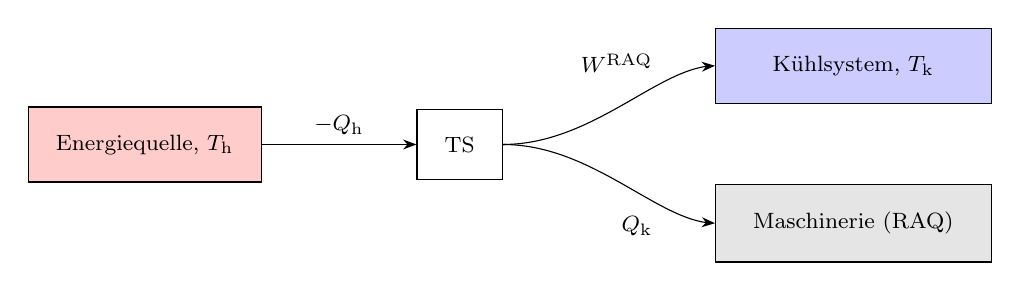
\begin{tikzpicture}
        [
            system node/.style={rectangle,draw,inner sep=10pt}
        ]
        \node[system node, fill=blue!20!white,minimum width=3.5cm] (RWQ) at (5,1) {Kühlsystem, $T_\mathrm{k}$};
        \node[system node, fill=black!10!white,minimum width=3.5cm] (RAQ) at (5,-1) {Maschinerie (RAQ)};
        \node[system node] (P) at (0,0) {TS};
        \draw[arr] (P) .. controls +(0:1.7) and +(180:.7) .. (RAQ.west) node[pos=.7,anchor=north east] {$\udiff Q_\mathrm{k}$};
        \draw[arr] (P) .. controls +(0:1.7) and +(180:.7) .. (RWQ.west) node[pos=.7,anchor=south east] {$\udiff W^\mathrm{RAQ}$};
        edge[arr] (RWQ) 
        edge[arr] (RAQ);
        \node[system node,align=center, fill=red!20!white] at (-4,0) {Energiequelle, $T_\mathrm{h}$} edge[arr] node[midway, above] {$-\udiff Q_\mathrm{h}$} (P);
    \end{tikzpicture}
}

% Maximized work in a coupled system
\newcommand{\tfigFridge}{
    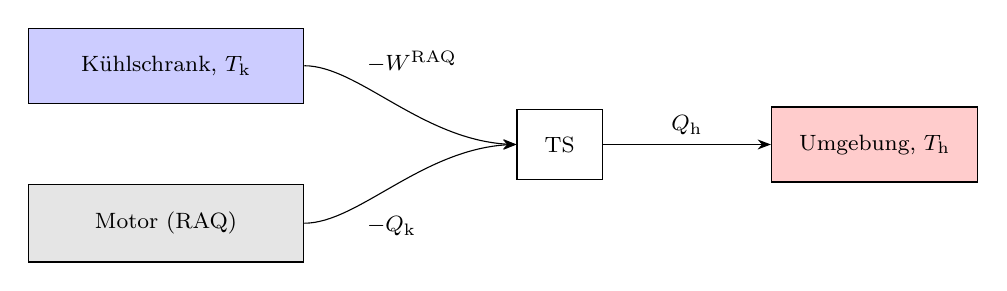
\begin{tikzpicture}
        [
            system node/.style={rectangle,draw,inner sep=10pt}
        ]
        \node[system node, fill=blue!20!white,minimum width=3.5cm] (RWQ) at (-5,1) {Kühlschrank, $T_\mathrm{k}$};
        \node[system node, fill=black!10!white,minimum width=3.5cm] (RAQ) at (-5,-1) {Motor (RAQ)};
        \node[system node] (P) at (0,0) {TS};
        \draw[rarr] (P) .. controls +(180:1.7) and +(0:.7) .. (RWQ.east) node[pos=.7,anchor=south west] {$-\udiff W^\mathrm{RAQ}$};
        \draw[rarr] (P) .. controls +(180:1.7) and +(0:.7) .. (RAQ.east) node[pos=.7,anchor=north west] {$-\udiff Q_\mathrm{k}$};
        edge[rarr] (RWQ) 
        edge[rarr] (RAQ);
        \node[system node,align=center, fill=red!20!white] at (4,0) {Umgebung, $T_\mathrm{h}$} edge[rarr] node[midway, above] {$\udiff Q_\mathrm{h}$} (P);
    \end{tikzpicture}
}

% Entropy-temperature diagram of the ideal carnot cycle
\newcommand{\tfigCarnotCycleIndicatorDiagram}{
    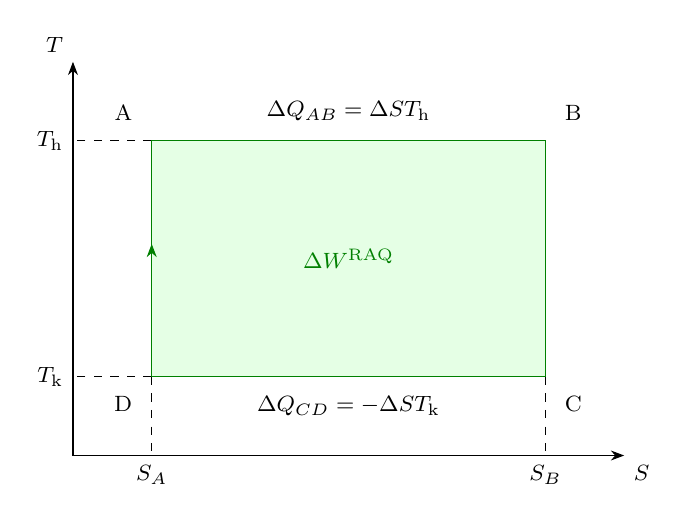
\begin{tikzpicture}
        \draw[arr] (0,0) -- (0,5) node[ylabel] {$T$};
        \draw[arr] (0,0) -- (7,0) node[xlabel] {$S$};
        
        \coordinate (A) at (1,4);
        \coordinate (B) at (6,4);
        \coordinate (C) at (6,1);
        \coordinate (D) at (1,1);
        
        \draw[dashed] (A) -- (0,4) node[left] {$T_\mathrm{h}$};
        \draw[dashed] (D) -- (0,1) node[left] {$T_\mathrm{k}$};
        \draw[dashed] (D) -- (1,0) node[below] {$S_A$};
        \draw[dashed] (C) -- (6,0) node[below] {$S_B$};
        
        \node[label={north west:A}] at (A) {};
        \node[label={north east:B}] at (B) {};
        \node[label={south east:C}] at (C) {};
        \node[label={south west:D}] at (D) {};
        
        \draw[midarrow=.1,nice green,fill=green!10!white] (D) rectangle (B) node[midway] {$\Delta W^{\mathrm{RAQ}}$};
        \node[label={north:$\Delta Q_{AB}=\Delta S T_\mathrm{h}$}] at ($(A)!.5!(B)$) {};
        \node[label={south:$\Delta Q_{CD}=-\Delta S T_\mathrm{k}$}] at ($(C)!.5!(D)$) {};
    \end{tikzpicture}
}